\section{Emil}

\setbeamertemplate{caption}{\raggedright\insertcaption\par}

\begin{frame}{Introduction}{Emil Már Einarsson\newline<eeinar14@student.aau.dk>}
	\begin{figure}[h!]
    	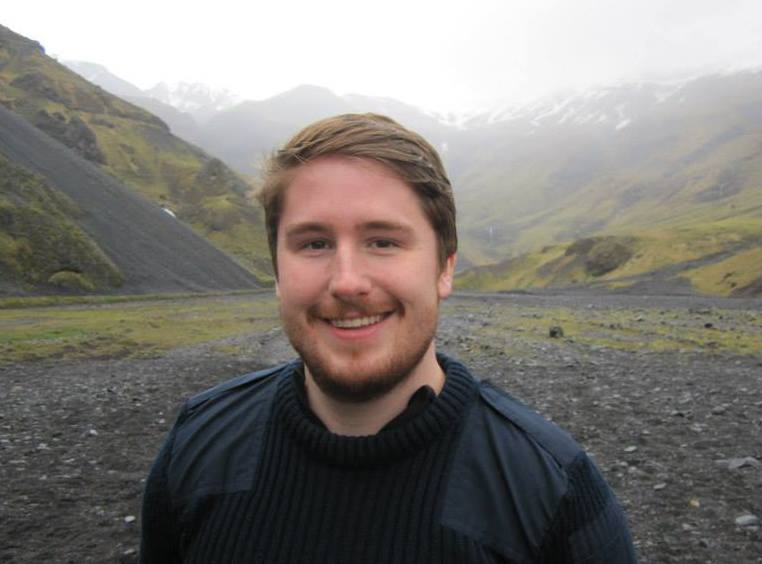
\includegraphics[width=0.5\textwidth]{images/emil.jpg}
    	\caption{Emil Már Einarsson}
		\centering    		
	\end{figure}
\end{frame}

\setbeamertemplate{caption}[default]

\begin{frame}{Hector SLAM}{Emil Már Einarsson\newline<eeinar14@student.aau.dk>}
  \begin{itemize}
  	\item Turning of laser too slow
  	\item Quality over quantity
  	\item Getting two system timed together
  	\item Design of a better housing
  	\item Future changes
  \end{itemize}
\end{frame}

\begin{frame}{Hector SLAM}{Emil Már Einarsson\newline<eeinar14@student.aau.dk>}
	\begin{figure}[h!]
    	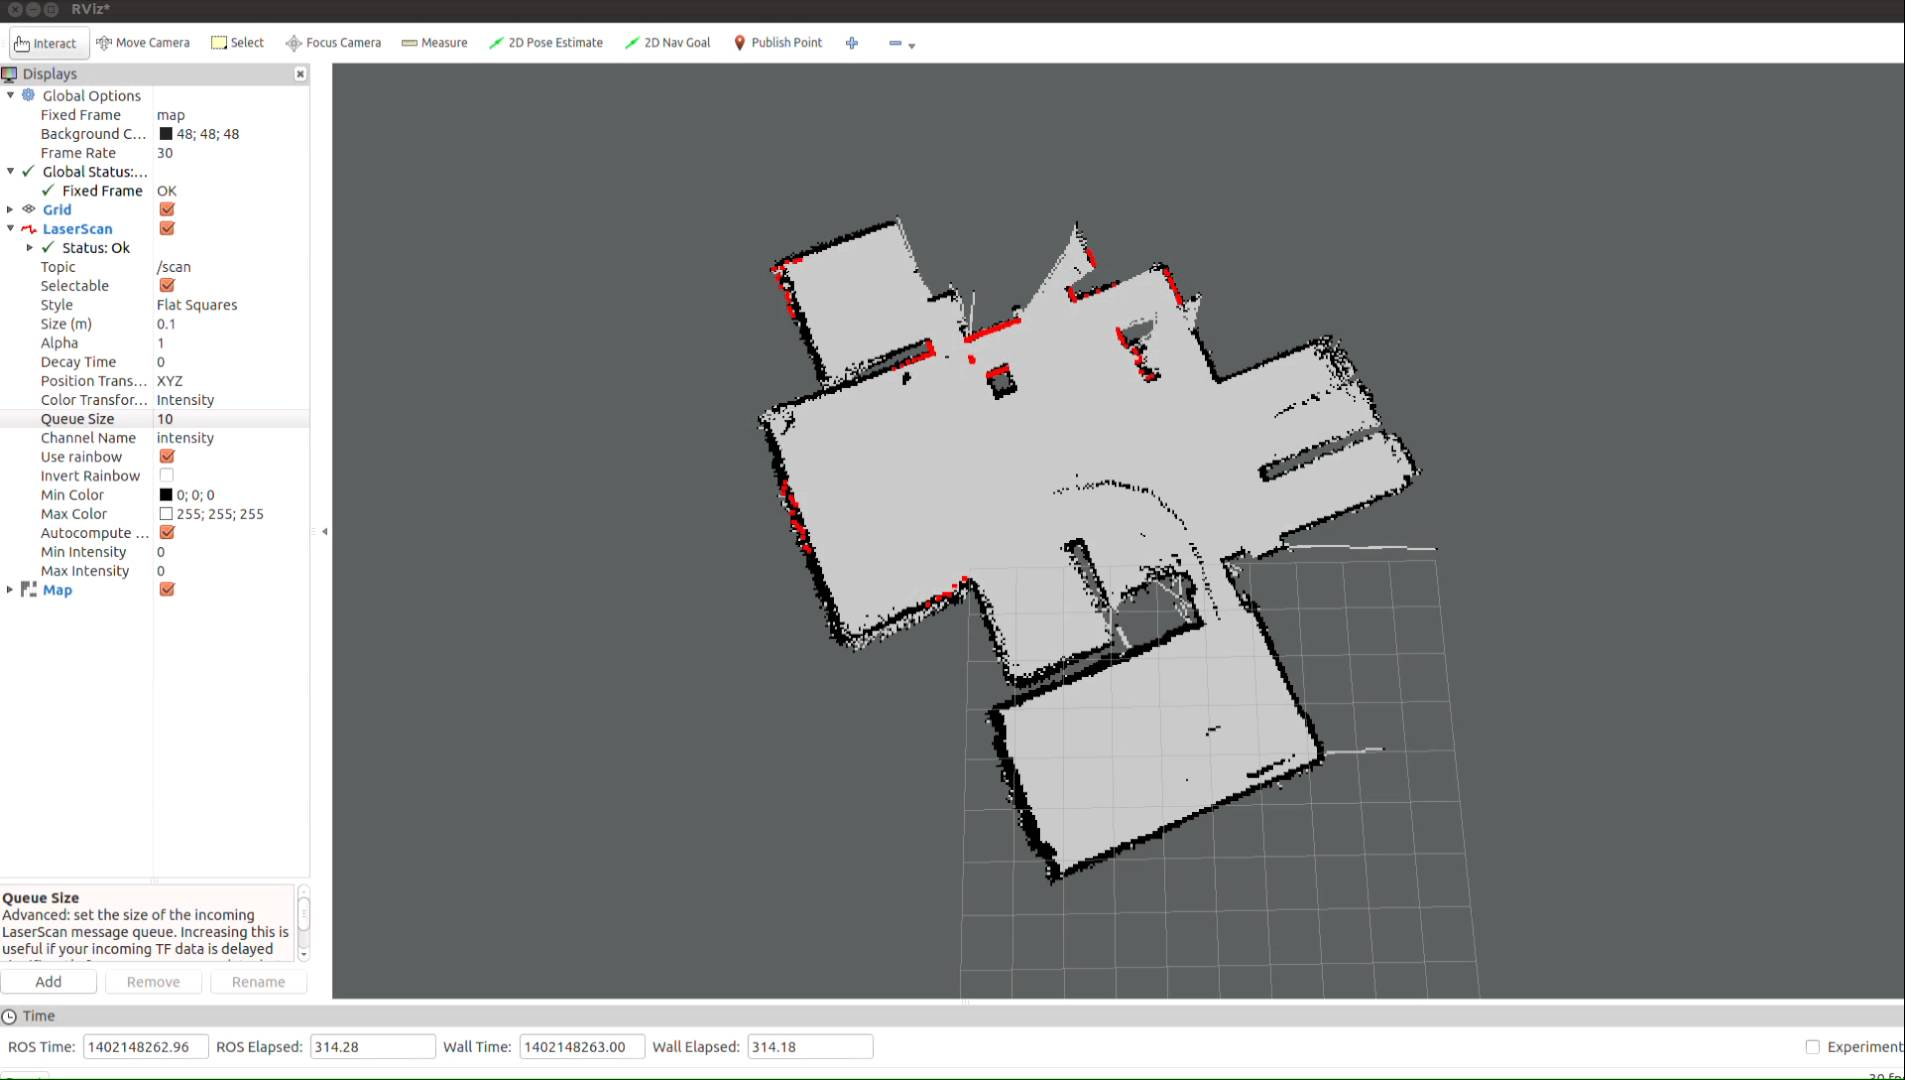
\includegraphics[width=0.8\textwidth]{images/hectorslam.jpg}
    	\caption{Full Hector Slam map}
    	\tiny{http://i.ytimg.com/vi/pCF7P7u8pDk/maxresdefault.jpg}
		\centering    		
	\end{figure}
\end{frame}

\begin{frame}{}{Emil Már Einarsson\newline<eeinar14@student.aau.dk>}
  \begin{itemize}
  	\item 1
  	\item 2
  	\item 3
  	\item 4
  	\item 5
  \end{itemize}
\end{frame}

\begin{frame}{}{Emil Már Einarsson\newline<eeinar14@student.aau.dk>}
	\begin{itemize}
		\item <2-> Mapping and Navigation of unknown terrain
		% Let's decode the title a bit and look at the individual parts a bit more in depth
		\begin{itemize}
			\item <3-> Mapping % idea behind, motivation, problem to solve
			\item <4-> Navigation % idea behind, motivation, problem to solve
			\item <5-> Unknown terrain % idea behind, motivation, problem to solve
		\end{itemize}
		\item <6-> 3D mapping, full autonomous navigation, etc. % what we have in plans for the future development of the idea (short-motivation)
	\end{itemize}
\end{frame}

\begin{frame}{3D mapping}{Emil Már Einarsson\newline<eeinar14@student.aau.dk>}
	\begin{figure}[h!]
    	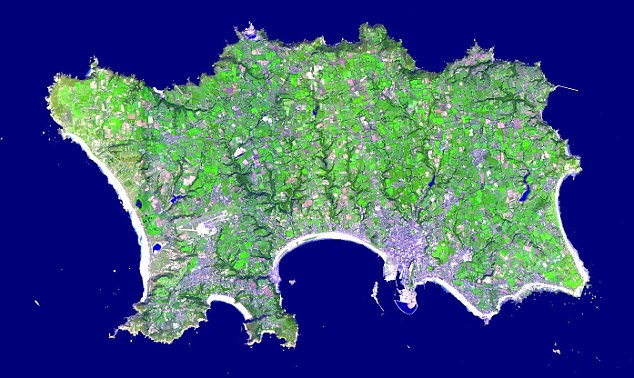
\includegraphics[width=0.8\textwidth]{images/3dmap2.jpg}
    	\caption{3D map overlay}
    	\tiny{http://www.dailymail.co.uk/sciencetech/article-2050967/Nasa-turns-exploring-planet-new-3D-map-outperforms-Google-Earth.html}
		\centering    		
	\end{figure}
\end{frame}

\begin{frame}{3D mapping}{Emil Már Einarsson\newline<eeinar14@student.aau.dk>}
	\begin{figure}[h!]
    	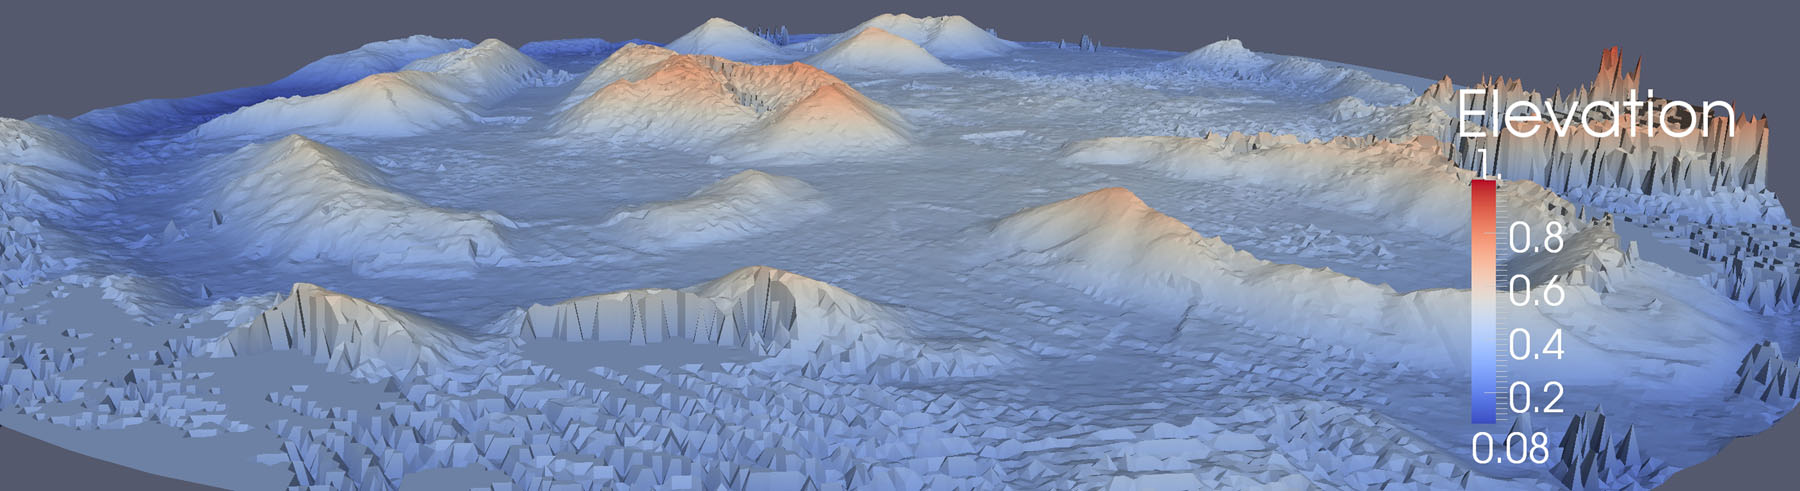
\includegraphics[width=1\textwidth]{images/3dmap1.jpg}
    	\caption{3D map elevation}
    	\tiny{http://asrl.utias.utoronto.ca/~cht/}
		\centering    		
	\end{figure}
\end{frame}


%pic1
%http://asrl.utias.utoronto.ca/~cht/

%pic2
%http://www.dailymail.co.uk/sciencetech/article-2050967/Nasa-turns-exploring-planet-new-3D-map-outperforms-Google-Earth.html

%hector slam pic
%http://i.ytimg.com/vi/pCF7P7u8pDk/maxresdefault.jpg


\setbeamertemplate{caption}[default]